\documentclass[10pt,a4paper]{article}
\usepackage[margin=2.2cm]{geometry}
\usepackage{amsmath,amssymb}
\usepackage{booktabs,tabularx,array,multirow}
\usepackage{xcolor}
\usepackage{tikz}
\usepackage{fancyhdr}
\usepackage{titlesec}
\usepackage{enumitem}
\usepackage[hidelinks]{hyperref}
\usepackage{tcolorbox}
\usepackage{float}

\definecolor{accent}{HTML}{1F4E79}
\definecolor{keybg}{HTML}{EEF3F6}
\definecolor{cmag}{HTML}{1F6F8B}
\definecolor{cfis}{HTML}{6A8F3A}
\definecolor{cgrad}{HTML}{C0612B}
\definecolor{crand}{HTML}{8A939C}

\newcommand{\best}[1]{\textcolor{cmag}{\textbf{#1}}}

\titleformat{\section}{\large\bfseries\color{accent}}{\thesection}{0.6em}{}
\titleformat{\subsection}{\normalsize\bfseries}{\thesubsection}{0.5em}{}
\setlist{itemsep=2pt,topsep=3pt}

\pagestyle{fancy}
\fancyhf{}
\fancyhead[L]{\small Reliable and Secure ReRAM Crossbar Accelerators}
\fancyhead[R]{\small CS5290 -- Phase 1 Results}
\fancyfoot[C]{\small\thepage}

\begin{document}

\begin{center}
{\small CS5290 Memory-Centric Computer Architecture $\cdot$ Results Report (24 October 2026)}\\[6pt]
{\LARGE\bfseries Protecting the Right Weights on a Noisy ReRAM Chip}\\[6pt]
{\large Phase 1 results for BERT-Base and DistilBERT on a hybrid SLC/MLC crossbar}
\end{center}

\begin{tcolorbox}[colback=keybg,colframe=accent,boxrule=0.5pt,arc=1pt,left=6pt,right=6pt,top=4pt,bottom=4pt,
  title={Main findings},fonttitle=\bfseries\small,coltitle=white]
\begin{enumerate}[leftmargin=*]
\item Storing a transformer only in dense two-bit cells (MLC) does not work: at realistic programming
noise, BERT-Base falls from 90\% to near coin-flip accuracy.
\item Keeping a small share of SVD components in reliable one-bit cells (SLC) recovers almost all of this
loss, but only if the right components are chosen.
\item Ranking components by their \textbf{singular value (magnitude)} is as good as the best placement we
could construct. A Fisher-information estimate of each component's expected damage on the chip reaches
the same accuracy (within one sentence in 872 on average over 600 chips), while a HyFlexPIM-style gradient
loses 3--12 points at high noise.
\item With magnitude ranking, 5--10\% SLC suffices at 5\% noise and about 30\% at 7.5\% noise, using
roughly 60--70\% of the memory cells of an all-SLC chip.
\item The conclusions hold on a more realistic chip (read noise, level-dependent noise, fixed ADC, IR drop),
and a 6-bit ADC is enough for a hybrid chip.
\item Stuck cells are the one problem placement cannot solve: all-MLC fails at 0.1\% stuck cells and
all-SLC at 1\%. This motivates fault-aware mapping, our next step.
\end{enumerate}
\end{tcolorbox}

\section{Problem and Questions}
A ReRAM crossbar computes a matrix--vector product inside memory: each weight is stored as the
conductance of resistive cells, and the currents of a column add up to the result. This avoids most of the
data movement of conventional hardware, but a cell cannot be programmed exactly, so every weight carries
random error. A cell can hold one bit (SLC), with two well-separated levels that tolerate noise, or two
bits (MLC), which is denser but more fragile. In our set-up an 8-bit weight needs 7 SLC or 4 MLC cells per
sign.

HyFlexPIM (ISCA 2025) splits each weight matrix with singular value decomposition (SVD) into components,
stores the most important ones in SLC and the rest in MLC, and ranks importance by the loss gradient. We
asked: (i) does this hybrid scheme hold up in a bit-accurate hardware simulation, (ii) which components
should be protected, and how many, and (iii) which hardware effects still break it.

\section{Method}
We used two pretrained sentiment classifiers, \textbf{BERT-Base} (72 weight matrices on the crossbar) and
\textbf{DistilBERT} (36), evaluated on all 872 validation sentences of SST-2. Each matrix is factorised
with SVD (384 components for a $768\times768$ layer) and the model is fine-tuned for 8 epochs. The
simulator stores 8-bit weights on differential cell pairs split into bit slices. Programming noise $\sigma$
is added to every cell as a fraction of the maximum conductance. One \emph{chip} is one random draw of all
cell errors; results are averaged over 5--20 chips, and we also report the worst chip. Every placement is
evaluated on the same chips, so differences between placements are not due to chance draws. The SVD model
is built once: a placement only decides which cells each component is stored in.

\subsection{Placements}
\begin{itemize}
\item \textbf{All SLC} and \textbf{All MLC}: the two extremes, giving the best and the cheapest chip.
\item \textbf{Random}: a share of components chosen at random, as a control.
\item \textbf{Magnitude}: the components with the largest singular values $\sigma_r$.
\item \textbf{Gradient (HyFlexPIM-style)}: $\sum_b |\partial L_b/\partial\sigma_r|$, absolute loss gradients
summed over batches of 32 training sentences with dropout on.
\item \textbf{Fisher}: the expected rise in loss if component $r$ is left in MLC,
\[
  D_r \;=\; \sum_{e\,\in\,\text{entries of } r} F_e\,\mathrm{Var}(\text{noise}_e),
\]
summed over every stored entry of the component (its row $\sigma_r v_r$ and its column $u_r$). $F_e$ is
the empirical Fisher information of entry $e$ over 2{,}048 training sentences, and the noise variance
follows our cell model: fixed cell noise becomes weight noise in proportion to the 8-bit scale of the
crossbar row that holds the entry.
\end{itemize}

\noindent Two design choices follow from how the chip behaves. The gradient takes absolute values per
batch, because on a trained model the gradients of individual sentences point in opposite directions and
would largely cancel in a single sum. The Fisher score covers every stored entry of a component, because
chip noise disturbs all of them, not only $\sigma_r$.

\section{Baseline: the Cost of SVD}

\begin{table}[h]
\centering\small
\begin{tabular}{@{}lcccc@{}}
\toprule
Model & Original FP32 & Original INT8 & SVD, before fine-tune & SVD, after fine-tune \\
\midrule
BERT-Base  & 92.43 & 91.86 & 89.33 & 90.14 \\
DistilBERT & 91.06 & 90.37 & 89.68 & 89.11 \\
\bottomrule
\end{tabular}
\caption{SST-2 accuracy (\%) with no hardware error.}
\end{table}

8-bit quantisation costs only about 0.6 points. SVD costs about 2 points even after fine-tuning; for
DistilBERT, 8 epochs slightly over-fitted (HyFlexPIM uses 1--3). This loss is paid before any hardware
error and applies equally to every placement. With no noise, the simulated chip matches the SVD model to
within 0.5 points for every placement, confirming that the simulator adds no hidden error.

\section{Programming Noise}

\begin{table}[h]
\centering\small
\begin{tabular}{@{}lcccccc@{}}
\toprule
Placement & $\sigma=0$ & 2\% & 3\% & 5\% & 7.5\% & 10\% \\
\midrule
All SLC & 89.9 & 89.3 & 89.1 & 87.8 & 85.9 & 79.7 \\
All MLC & 90.0 & 87.3 & 83.9 & 66.3 & 52.2 & 51.3 \\
\midrule
Magnitude, 20\% SLC & 89.7 & 89.9 & \best{90.0} & 88.6 & 83.5 & 72.0 \\
Fisher, 20\% SLC    & 89.1 & 90.1 & \best{90.0} & \best{89.0} & \best{84.5} & \best{73.7} \\
Gradient, 20\% SLC  & 89.8 & \best{90.2} & \best{90.0} & 88.0 & 79.3 & 67.7 \\
Random, 20\% SLC    & 90.0 & 89.9 & 87.7 & 78.8 & 58.8 & 49.1 \\
\bottomrule
\end{tabular}
\caption{BERT-Base, mean accuracy (\%) over 5 chips. DistilBERT behaves the same way (Appendix~A).}
\end{table}

All-MLC collapses once noise reaches 5\%. Protecting 20\% of the components by magnitude or Fisher
recovers nearly all of the loss, the gradient recovers less at high noise, and a random 20\% recovers
little: \emph{which} components are protected matters more than how many.

\section{Choosing and Sizing the Protected Set}

\begin{figure}[h]
\centering
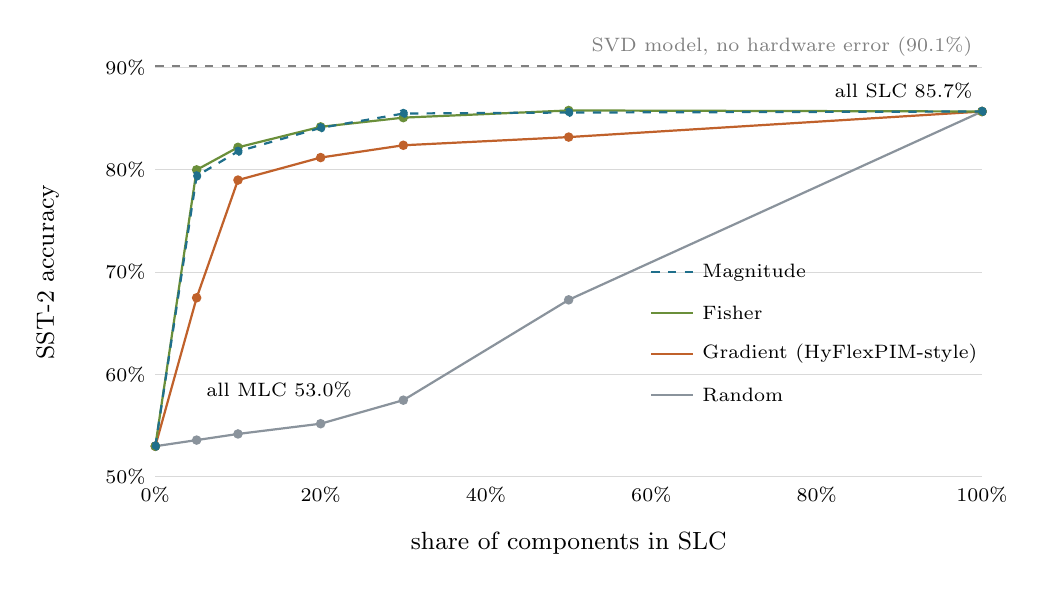
\begin{tikzpicture}[x=0.105cm,y=0.13cm]
  \foreach \v in {50,60,70,80,90} {
    \draw[gray!30] (0,\v-50) -- (100,\v-50);
    \node[left,font=\scriptsize] at (0,\v-50) {\v\%};
  }
  \foreach \v in {0,20,40,60,80,100}
    \node[below,font=\scriptsize] at (\v,0) {\v\%};
  \node[font=\small] at (50,-6.5) {share of components in SLC};
  \node[rotate=90,font=\small] at (-13,20) {SST-2 accuracy};
  \draw[gray,dashed] (0,40.14) -- (100,40.14);
  \node[above left,font=\scriptsize,gray] at (100,40.14) {SVD model, no hardware error (90.1\%)};
  \draw[crand,thick] plot[mark=*,mark size=1.3pt] coordinates
    {(0,3.0) (5,3.6) (10,4.2) (20,5.2) (30,7.5) (50,17.3) (100,35.7)};
  \draw[cgrad,thick] plot[mark=*,mark size=1.3pt] coordinates
    {(0,3.0) (5,17.5) (10,29.0) (20,31.2) (30,32.4) (50,33.2) (100,35.7)};
  \draw[cfis,thick] plot[mark=*,mark size=1.3pt] coordinates
    {(0,3.0) (5,30.0) (10,32.2) (20,34.2) (30,35.1) (50,35.8) (100,35.7)};
  \draw[cmag,thick,dashed] plot[mark=*,mark size=1.3pt] coordinates
    {(0,3.0) (5,29.4) (10,31.8) (20,34.1) (30,35.5) (50,35.6) (100,35.7)};
  \node[right,font=\scriptsize] at (5,8.5) {all MLC 53.0\%};
  \node[above left,font=\scriptsize] at (100,36.0) {all SLC 85.7\%};
  \begin{scope}[shift={(60,8)},font=\scriptsize]
    \draw[cmag,thick,dashed] (0,12) -- (5,12); \node[right] at (5,12) {Magnitude};
    \draw[cfis,thick] (0,8) -- (5,8);   \node[right] at (5,8) {Fisher};
    \draw[cgrad,thick] (0,4) -- (5,4);  \node[right] at (5,4) {Gradient (HyFlexPIM-style)};
    \draw[crand,thick] (0,0) -- (5,0);  \node[right] at (5,0) {Random};
  \end{scope}
\end{tikzpicture}
\caption{BERT-Base at $\sigma=7.5\%$, mean of 20 chips. 0\% and 100\% are all-MLC and all-SLC.
Magnitude (dashed) and Fisher lie on top of each other.}
\end{figure}

\begin{table}[h]
\centering\small
\begin{tabular}{@{}llccccccc@{}}
\toprule
Noise & Placement & 0\% & 5\% & 10\% & 20\% & 30\% & 50\% & 100\% \\
\midrule
\multirow{4}{*}{$\sigma=5\%$}
 & Magnitude & \multirow{4}{*}{66.8} & \best{88.0} & \best{88.6} & 88.7 & \best{88.9} & \best{88.9} & \multirow{4}{*}{88.0} \\
 & Fisher    & & 87.9 & \best{88.6} & \best{88.8} & \best{88.9} & \best{88.9} & \\
 & Gradient  & & 84.2 & 88.2 & 88.4 & 88.4 & 88.1 & \\
 & Random    & & 72.5 & 73.6 & 76.2 & 77.8 & 83.4 & \\
\midrule
\multirow{4}{*}{$\sigma=7.5\%$}
 & Magnitude & \multirow{4}{*}{53.0} & 79.4 & 81.8 & 84.1 & \best{85.5} & 85.6 & \multirow{4}{*}{85.7} \\
 & Fisher    & & \best{80.0} & \best{82.2} & \best{84.2} & 85.1 & \best{85.8} & \\
 & Gradient  & & 67.5 & 79.0 & 81.2 & 82.4 & 83.2 & \\
 & Random    & & 53.6 & 54.2 & 55.2 & 57.5 & 67.3 & \\
\bottomrule
\end{tabular}
\caption{BERT-Base, mean accuracy (\%) over 20 chips by share of components in SLC. DistilBERT,
$\sigma=3\%$ and worst-chip results are in Appendix~A.}
\end{table}

\subsection{Magnitude and Fisher are equivalent; the gradient falls behind}
Because every placement is tested on the same 20 chips, we can compare them chip by chip. Over all 300
chips of the SLC-share study (3 noise levels, 5 SLC shares), Fisher differs from magnitude by
$+0.4\pm0.7$ sentences per chip on BERT-Base and $-0.6\pm0.7$ on DistilBERT (mean $\pm$ standard error,
out of 872): no measurable difference. The gradient is clearly worse, by $17.3\pm2.0$ and $7.8\pm1.1$
sentences; at $\sigma=7.5\%$ it trails by 3 points with 20\% SLC and by 12 points with 5\% SLC. Random selection is far behind everywhere.

\subsection{Why magnitude is enough}
After SVD, component $r$ is stored as the row $\sigma_r v_r$ and the column $u_r$. Each row is quantised
with its own scale, set by its largest value, so the same cell noise produces a weight error proportional
to $\sigma_r$. The harm a component does when left in MLC is its sensitivity times the size of the noise
it receives, and the Fisher score estimates exactly this product over all of the component's stored
entries. That this principled estimate ends up choosing essentially the same components as magnitude
shows that noise size, set by $\sigma_r$, dominates the damage: magnitude ranking is close to the best
placement available under this noise model. It also needs no data or gradients. The gradient falls short
because it measures sensitivity to small changes of $\sigma_r$ alone, ignoring both the size of the noise
and the other stored entries.

\subsection{How much SLC is needed}
With magnitude ranking, the SLC share needed to come within half a point of an all-SLC chip is about 5\%
at $\sigma=3\%$, 5--10\% at $\sigma=5\%$ and about 30\% at $\sigma=7.5\%$; DistilBERT needs 30--50\% at
$\sigma=7.5\%$. Counting only weight cells, a share $f$ in SLC needs $7f+4(1-f)$ cells per weight against 7
for all-SLC: 61\% of the cells at 10\% SLC and 70\% at 30\% (all-MLC: 57\%). At moderate noise a hybrid
chip therefore approaches MLC density at SLC accuracy.

\section{Stuck-At Faults}
A stuck cell reads fully on or fully off, whatever was written. We made a share of all cells stuck, half
on and half off, with no programming noise and 20\% SLC.

\begin{table}[h]
\centering\small
\begin{tabular}{@{}lccccccc@{}}
\toprule
Placement & 0\% & 0.1\% & 0.2\% & 0.5\% & 1\% & 2\% & 5\% \\
\midrule
All SLC & 89.9 & 88.3 & 85.6 & \best{79.0} & \best{62.7} & 51.4 & 49.6 \\
All MLC & 90.0 & 58.6 & 52.6 & 50.8 & 51.2 & 49.6 & 49.6 \\
\midrule
Magnitude, 20\% SLC & 89.7 & 89.6 & \best{88.6} & 76.8 & 57.9 & 51.0 & 50.0 \\
Fisher, 20\% SLC    & 89.1 & \best{89.7} & 88.4 & 75.6 & 55.5 & 49.5 & 50.3 \\
Gradient, 20\% SLC  & 89.8 & 89.4 & 87.5 & 71.0 & 52.8 & 50.2 & 49.5 \\
Random, 20\% SLC    & 90.0 & 67.9 & 55.8 & 50.7 & 50.6 & 50.2 & 49.9 \\
\bottomrule
\end{tabular}
\caption{BERT-Base, mean accuracy (\%) over 20 chips versus the share of stuck cells.}
\end{table}

Faults are far more harmful than noise, because a stuck cell in a high-order slice shifts its weight by a
large, fixed amount. All-MLC fails when one cell in a thousand is stuck, and even all-SLC fails at 1\%. Up
to 0.2\%, magnitude and Fisher with 20\% SLC are as good as all-SLC; the gradient degrades sooner. Near
the collapse point, accuracy varies by 6--9 points from chip to chip, so survival depends on \emph{where}
the faults land. Reported stuck-cell rates for real arrays are of the order of a few percent, well past
the point where every placement fails, so fault-aware mapping is required.

\section{A More Realistic Chip}
We added the main effects missing from the basic simulator and tested each on its own, after checking the
new simulator against exact results.

\begin{table}[h]
\centering\small
\begin{tabular}{@{}lccccc@{}}
\toprule
Condition & All SLC & All MLC & Magnitude & Fisher & Gradient \\
\midrule
No non-idealities & 89.7 & 90.4 & 90.6 & 89.6 & 90.3 \\
Read noise 2\% (fresh at every read) & 89.0 & 77.3 & \best{90.1} & 89.7 & 89.8 \\
Read noise 5\% & 80.0 & 53.0 & 82.5 & \best{82.7} & 76.6 \\
Middle MLC levels $2\times$ noisier ($\sigma=5\%$) & 88.2 & 62.5 & \best{88.4} & \best{88.4} & 87.8 \\
1\% stuck cells, scattered & \best{61.3} & 50.7 & 56.4 & 55.6 & 52.6 \\
1\% stuck cells, $3\times3$ clusters & \best{66.7} & 50.8 & 54.0 & 53.1 & 51.5 \\
1\% stuck cells, whole bit lines & \best{57.0} & 50.4 & 50.4 & 52.2 & 51.0 \\
Fixed ADC with bit-serial inputs, 6 bits & 89.3 & 83.0 & 90.0 & \best{90.5} & 89.6 \\
Fixed ADC with bit-serial inputs, 5 bits & 51.1 & 51.1 & 51.1 & 51.6 & 53.0 \\
IR drop, $r=3\times10^{-4}$ & 88.9 & 89.8 & 90.4 & \best{91.1} & 90.5 \\
IR drop, $r=3\times10^{-3}$ & 58.5 & \best{79.1} & 76.8 & 72.8 & 76.4 \\
\bottomrule
\end{tabular}
\caption{BERT-Base, mean accuracy (\%); hybrids keep 20\% of components in SLC. Digital SVD model:
90.1\%. $r$ is the resistance of one wire segment relative to a cell's on-resistance. DistilBERT results
are in Appendix~A.}
\end{table}

\begin{itemize}
\item \textbf{Read noise and level-dependent noise} behave like programming noise: all-MLC fails, while
magnitude and Fisher stay within about a point of all-SLC. The gradient loses 6 points at 5\% read noise.
\item \textbf{ADC resolution.} With the ADC range fixed by calibration, 6 bits is enough for all-SLC and the
hybrids, all-MLC needs 7 bits, and 5 bits fails for every placement. With 5\% programming noise
(DistilBERT), 6 bits still holds the magnitude hybrid at 88.5\% while all-MLC drops to 56.0\%. Since ADCs
dominate crossbar energy, this sets the target for the hardware-cost study.
\item \textbf{IR drop} has no effect at realistic wire resistance ($r\lesssim3\times10^{-4}$ in
$128\times128$ tiles). When large, it hurts SLC most: an SLC cell storing a 1 sits at full conductance and
loses the most current to wire resistance.
\item \textbf{Fault patterns.} Clustered faults affect fewer weights than scattered ones, and whole broken
bit lines are worst. At 1\% every placement is already near failure, confirming Section~6.
\end{itemize}
Random selection was not repeated for these effects: as a control, it is already far behind in every
experiment above.

\section{Relation to HyFlexPIM}
Our results agree with HyFlexPIM that a hybrid SLC/MLC layout works, but not on how to rank components.
HyFlexPIM reports that its gradient ranking beats ranking by singular value by about a point or less, on
MRPC and CoLA at a single noise level. We find no difference at mild noise ($\sigma=3\%$) and the reverse
at high noise, so the two findings need not conflict. Three differences in set-up matter:
\begin{itemize}
\item \textbf{Noise model.} HyFlexPIM applies relative noise to whole weights, $\tilde W=W\odot(1+\eta)$, so
small weights are almost exact. We add noise to each cell, as real hardware and standard simulators do,
so even a zero weight carries the error of its two drifting cells. The paper gives no reason for its choice;
its citations support only the noise level, a 4.04\% bit error rate measured on 3 million real MLC cells,
which is itself a per-cell quantity.
\item \textbf{Noise range.} The paper evaluates one fixed noise level. Our sweeps cover 2--10\%, and the
ranking differences appear only at $\sigma\geq5\%$.
\item \textbf{When gradients are taken.} HyFlexPIM records gradients during fine-tuning; ours are taken on
the trained model. A re-run of their fine-tuning was not pursued, since magnitude already matches the
best placement we could construct.
\end{itemize}

\section{Conclusions}
\begin{itemize}
\item A hybrid SLC/MLC layout is necessary: all-MLC storage fails at realistic noise.
\item Ranking components by singular value is the recommended placement. A Fisher estimate of each
component's expected damage chooses essentially the same components and reaches the same accuracy, which
shows that magnitude is close to the best placement under this noise model; it needs no data or
gradients. A HyFlexPIM-style gradient is clearly weaker at high noise.
\item The SLC share should follow the expected noise: about 10\% at moderate noise and 30\% at high noise,
saving 30--40\% of the cells of an all-SLC chip.
\item The conclusions hold under read noise, level-dependent noise, a fixed 6-bit ADC and realistic IR drop.
\item Stuck cells break every placement at rates below those reported for real arrays, so fault-aware
mapping is necessary, not optional.
\end{itemize}

\section{Limitations}
\begin{itemize}
\item Each non-ideality was tested on its own; their combined effect is not yet measured. The IR-drop model
is static, and the ADC range is set by the maximum calibration value rather than a percentile.
\item Inputs are quantised to 8 bits with one scale per batch of sentences, so accuracy shifts slightly
with batch size (by up to about one point without noise). All placements within an experiment use the same
batches, so comparisons are unaffected; per-sentence input scaling will be added.
\item The SVD step costs about 2 points, and DistilBERT's fine-tuning needs early stopping.
\item All results are on SST-2; MRPC and the CNN models follow in Phase 2. Literature figures for stuck-cell
rates and wire resistance are still to be confirmed with citations.
\end{itemize}

\section{Next Steps}
Stuck cells are the one effect placement cannot handle. Fault-aware mapping, and its extension that
jointly accounts for cell type, faults and IR drop, come next; they need no retraining, only a smarter
assignment of components to crossbar positions. Noise-aware training, including a variant that applies
SLC- and MLC-specific noise during fine-tuning, follows.

\vspace{6pt}
\noindent{\footnotesize\color{gray} Models: textattack/bert-base-uncased-SST-2 and
distilbert-base-uncased-finetuned-sst-2-english. Simulator: 8-bit weights, on/off ratio 100, differential
cell pairs, $128\times128$ tiles. Ranking scores computed on 2{,}048 SST-2 training sentences.}

\clearpage
\appendix
\section{Complete Result Tables}
All values are SST-2 validation accuracy (\%, 872 sentences). Hybrid placements keep 20\% of components in
SLC unless the SLC share is varied. In each column the best hybrid placement is shown in colour; ``--''
marks points that were not run.

\subsection{Programming noise (5 chips)}

\begin{table}[H]
\centering\small
\begin{tabular}{@{}lccccccc@{}}
\toprule
Placement & 0 & 1\% & 2\% & 3\% & 5\% & 7.5\% & 10\% \\
\midrule
All SLC & 89.9 & 89.6 & 89.3 & 89.1 & 87.8 & 85.9 & 79.7 \\
All MLC & 90.0 & 89.3 & 87.3 & 83.9 & 66.3 & 52.2 & 51.3 \\
\midrule
Magnitude & 89.7 & 89.8 & 89.9 & 90.0 & 88.6 & 83.5 & 72.0 \\
Fisher & 89.1 & 89.7 & 90.1 & \best{90.0} & \best{89.0} & \best{84.5} & \best{73.7} \\
Gradient & 89.8 & \best{90.4} & \best{90.2} & 90.0 & 88.0 & 79.3 & 67.7 \\
Random & \best{90.0} & 90.1 & 89.9 & 87.7 & 78.8 & 58.8 & 49.1 \\
\bottomrule
\end{tabular}
\caption{BERT-Base, mean accuracy versus programming noise $\sigma$.}
\end{table}

\begin{table}[H]
\centering\small
\begin{tabular}{@{}lccccccc@{}}
\toprule
Placement & 0 & 1\% & 2\% & 3\% & 5\% & 7.5\% & 10\% \\
\midrule
All SLC & 89.0 & 88.7 & 88.8 & 88.6 & 88.5 & 87.5 & 85.9 \\
All MLC & 89.1 & 88.4 & 87.9 & 86.1 & 74.5 & 60.4 & 56.0 \\
\midrule
Magnitude & 89.1 & 88.9 & 88.9 & 88.9 & 88.4 & \best{85.9} & \best{77.7} \\
Fisher & 89.0 & \best{89.0} & \best{89.0} & \best{89.1} & \best{88.5} & 85.5 & 77.6 \\
Gradient & \best{89.8} & 88.5 & 88.9 & 88.7 & 87.7 & 83.4 & 69.8 \\
Random & 88.6 & 88.7 & 88.7 & 87.8 & 82.8 & 61.8 & 52.4 \\
\bottomrule
\end{tabular}
\caption{DistilBERT, mean accuracy versus programming noise $\sigma$.}
\end{table}

\subsection{Accuracy versus SLC share (mean of 20 chips)}

\begin{table}[H]
\centering\small
\begin{tabular}{@{}llccccccc@{}}
\toprule
Noise & Placement & 0\% & 5\% & 10\% & 20\% & 30\% & 50\% & 100\% \\
\midrule
\multirow{4}{*}{3\%} & Magnitude & \multirow{4}{*}{82.1} & \best{89.7} & 89.9 & 89.8 & 89.8 & 89.7 & \multirow{4}{*}{89.2} \\
 & Fisher &  & 89.6 & 89.8 & 89.8 & 89.8 & \best{89.8} &  \\
 & Gradient &  & 88.7 & \best{90.0} & \best{90.0} & \best{89.9} & 89.6 &  \\
 & Random &  & 87.0 & 86.9 & 87.6 & 87.3 & 89.0 &  \\
\midrule
\multirow{4}{*}{5\%} & Magnitude & \multirow{4}{*}{66.8} & \best{88.0} & 88.6 & 88.7 & \best{88.9} & 88.9 & \multirow{4}{*}{88.0} \\
 & Fisher &  & 87.9 & \best{88.6} & \best{88.8} & 88.9 & \best{88.9} &  \\
 & Gradient &  & 84.2 & 88.2 & 88.4 & 88.4 & 88.1 &  \\
 & Random &  & 72.5 & 73.6 & 76.2 & 77.8 & 83.4 &  \\
\midrule
\multirow{4}{*}{7.5\%} & Magnitude & \multirow{4}{*}{53.0} & 79.4 & 81.8 & 84.1 & \best{85.5} & 85.6 & \multirow{4}{*}{85.7} \\
 & Fisher &  & \best{80.0} & \best{82.2} & \best{84.2} & 85.1 & \best{85.8} &  \\
 & Gradient &  & 67.5 & 79.0 & 81.2 & 82.4 & 83.2 &  \\
 & Random &  & 53.6 & 54.2 & 55.2 & 57.5 & 67.3 &  \\
\bottomrule
\end{tabular}
\caption{BERT-Base, mean accuracy by share of components in SLC (0\% = all MLC, 100\% = all SLC).}
\end{table}

\begin{table}[H]
\centering\small
\begin{tabular}{@{}llccccccc@{}}
\toprule
Noise & Placement & 0\% & 5\% & 10\% & 20\% & 30\% & 50\% & 100\% \\
\midrule
\multirow{4}{*}{3\%} & Magnitude & \multirow{4}{*}{86.0} & 88.4 & 88.6 & \best{88.8} & \best{88.9} & 88.7 & \multirow{4}{*}{88.7} \\
 & Fisher &  & \best{88.5} & \best{88.7} & 88.7 & 88.8 & 88.6 &  \\
 & Gradient &  & 88.4 & 88.5 & 88.6 & 88.8 & \best{88.7} &  \\
 & Random &  & 86.4 & 86.8 & 87.5 & 88.1 & 88.4 &  \\
\midrule
\multirow{4}{*}{5\%} & Magnitude & \multirow{4}{*}{74.8} & \best{87.4} & \best{88.0} & 88.1 & \best{88.8} & \best{88.4} & \multirow{4}{*}{88.2} \\
 & Fisher &  & 87.3 & 87.8 & \best{88.4} & 88.1 & 88.3 &  \\
 & Gradient &  & 87.3 & 87.3 & 87.7 & 88.1 & 87.8 &  \\
 & Random &  & 75.4 & 77.4 & 81.9 & 82.3 & 85.7 &  \\
\midrule
\multirow{4}{*}{7.5\%} & Magnitude & \multirow{4}{*}{56.9} & 80.2 & \best{84.0} & 85.2 & \best{86.6} & 86.9 & \multirow{4}{*}{87.4} \\
 & Fisher &  & \best{80.8} & 83.8 & \best{85.4} & 86.0 & \best{87.0} &  \\
 & Gradient &  & 78.0 & 80.7 & 83.1 & 84.8 & 86.0 &  \\
 & Random &  & 56.4 & 58.2 & 63.1 & 64.7 & 73.7 &  \\
\bottomrule
\end{tabular}
\caption{DistilBERT, mean accuracy by share of components in SLC (0\% = all MLC, 100\% = all SLC).}
\end{table}

\subsection{Accuracy versus SLC share (worst of 20 chips)}

\begin{table}[H]
\centering\small
\begin{tabular}{@{}llccccccc@{}}
\toprule
Noise & Placement & 0\% & 5\% & 10\% & 20\% & 30\% & 50\% & 100\% \\
\midrule
\multirow{4}{*}{3\%} & Magnitude & \multirow{4}{*}{70.9} & \best{88.9} & \best{89.2} & 88.9 & 88.9 & 88.5 & \multirow{4}{*}{87.7} \\
 & Fisher &  & 88.5 & 88.9 & 88.6 & \best{89.1} & \best{88.8} &  \\
 & Gradient &  & 87.5 & 89.2 & \best{89.2} & 88.9 & 88.5 &  \\
 & Random &  & 83.9 & 82.2 & 85.7 & 84.4 & 86.0 &  \\
\midrule
\multirow{4}{*}{5\%} & Magnitude & \multirow{4}{*}{51.6} & \best{86.4} & \best{87.6} & \best{88.0} & \best{88.1} & 86.9 & \multirow{4}{*}{85.8} \\
 & Fisher &  & 86.2 & 87.0 & 87.8 & 87.7 & \best{87.4} &  \\
 & Gradient &  & 77.3 & 86.5 & 86.9 & 86.5 & 85.4 &  \\
 & Random &  & 57.8 & 61.5 & 63.5 & 52.4 & 70.9 &  \\
\midrule
\multirow{4}{*}{7.5\%} & Magnitude & \multirow{4}{*}{49.1} & \best{73.4} & \best{76.8} & 76.0 & \best{82.1} & \best{83.0} & \multirow{4}{*}{82.3} \\
 & Fisher &  & 72.2 & 72.5 & \best{78.4} & 81.4 & 82.9 &  \\
 & Gradient &  & 52.3 & 72.8 & 75.8 & 70.0 & 76.6 &  \\
 & Random &  & 49.2 & 50.6 & 50.9 & 49.1 & 49.3 &  \\
\bottomrule
\end{tabular}
\caption{BERT-Base, worst-chip accuracy by share of components in SLC (0\% = all MLC, 100\% = all SLC).}
\end{table}

\begin{table}[H]
\centering\small
\begin{tabular}{@{}llccccccc@{}}
\toprule
Noise & Placement & 0\% & 5\% & 10\% & 20\% & 30\% & 50\% & 100\% \\
\midrule
\multirow{4}{*}{3\%} & Magnitude & \multirow{4}{*}{83.6} & \best{87.7} & \best{87.4} & 87.3 & 88.0 & \best{87.7} & \multirow{4}{*}{87.5} \\
 & Fisher &  & 87.7 & 87.4 & \best{87.6} & 87.8 & 87.5 &  \\
 & Gradient &  & 87.6 & 87.3 & 87.2 & \best{88.1} & 87.3 &  \\
 & Random &  & 84.3 & 84.1 & 85.9 & 87.3 & 86.5 &  \\
\midrule
\multirow{4}{*}{5\%} & Magnitude & \multirow{4}{*}{62.3} & 85.6 & \best{86.0} & 85.7 & \best{87.3} & \best{87.5} & \multirow{4}{*}{86.8} \\
 & Fisher &  & 85.8 & 86.0 & \best{86.5} & 87.0 & 86.8 &  \\
 & Gradient &  & \best{85.9} & 85.8 & 85.8 & 86.1 & 85.4 &  \\
 & Random &  & 67.3 & 67.4 & 77.8 & 63.2 & 77.3 &  \\
\midrule
\multirow{4}{*}{7.5\%} & Magnitude & \multirow{4}{*}{50.1} & 72.5 & \best{79.5} & 82.8 & 83.4 & 85.0 & \multirow{4}{*}{85.9} \\
 & Fisher &  & \best{76.3} & 79.5 & \best{83.6} & \best{83.8} & \best{85.9} &  \\
 & Gradient &  & 72.9 & 73.3 & 79.9 & 83.4 & 84.4 &  \\
 & Random &  & 50.8 & 50.7 & 52.1 & 50.9 & 54.5 &  \\
\bottomrule
\end{tabular}
\caption{DistilBERT, worst-chip accuracy by share of components in SLC (0\% = all MLC, 100\% = all SLC).}
\end{table}

\subsection{Stuck-at faults (20 chips)}

\begin{table}[H]
\centering\small
\begin{tabular}{@{}lccccccc@{}}
\toprule
Placement & 0 & 0.1\% & 0.2\% & 0.5\% & 1\% & 2\% & 5\% \\
\midrule
\multicolumn{8}{@{}l}{\emph{mean}} \\
All SLC & 89.9 & 88.3 & 85.6 & 79.0 & 62.7 & 51.4 & 49.6 \\
All MLC & 90.0 & 58.6 & 52.6 & 50.8 & 51.2 & 49.6 & 49.6 \\
\midrule
Magnitude & 89.7 & 89.6 & \best{88.6} & \best{76.8} & \best{57.9} & \best{51.0} & 50.0 \\
Fisher & 89.1 & \best{89.7} & 88.4 & 75.6 & 55.5 & 49.5 & \best{50.3} \\
Gradient & 89.8 & 89.4 & 87.5 & 71.0 & 52.8 & 50.2 & 49.5 \\
Random & \best{90.0} & 67.9 & 55.8 & 50.7 & 50.6 & 50.2 & 49.9 \\
\midrule
\multicolumn{8}{@{}l}{\emph{worst chip}} \\
All SLC & 89.9 & 83.0 & 71.3 & 57.5 & 50.9 & 49.1 & 41.3 \\
All MLC & 90.0 & 49.1 & 49.1 & 48.9 & 48.9 & 46.3 & 48.3 \\
\midrule
Magnitude & 89.7 & \best{89.1} & \best{86.2} & \best{66.2} & \best{50.8} & 47.0 & 46.2 \\
Fisher & 89.1 & 88.1 & 86.1 & 57.7 & 49.1 & 44.8 & \best{47.6} \\
Gradient & 89.8 & 85.9 & 82.1 & 53.6 & 49.1 & 46.7 & 47.4 \\
Random & \best{90.0} & 50.8 & 49.1 & 47.4 & 48.9 & \best{48.6} & 46.2 \\
\bottomrule
\end{tabular}
\caption{BERT-Base, accuracy versus share of stuck cells.}
\end{table}

\begin{table}[H]
\centering\small
\begin{tabular}{@{}lccccccc@{}}
\toprule
Placement & 0 & 0.1\% & 0.2\% & 0.5\% & 1\% & 2\% & 5\% \\
\midrule
\multicolumn{8}{@{}l}{\emph{mean}} \\
All SLC & 89.0 & 88.2 & 87.8 & 85.2 & 74.6 & 58.5 & 51.5 \\
All MLC & 89.1 & 65.5 & 58.2 & 52.3 & 51.1 & 50.2 & 49.4 \\
\midrule
Magnitude & 89.1 & \best{88.3} & \best{87.4} & 80.3 & \best{62.1} & \best{51.4} & 49.9 \\
Fisher & 89.0 & 88.3 & 87.2 & \best{80.3} & 62.1 & 51.3 & 50.4 \\
Gradient & \best{89.8} & 88.1 & 86.7 & 74.5 & 55.4 & 51.0 & \best{50.5} \\
Random & 88.6 & 76.9 & 63.3 & 51.3 & 51.0 & 49.4 & 50.1 \\
\midrule
\multicolumn{8}{@{}l}{\emph{worst chip}} \\
All SLC & 89.0 & 86.9 & 85.3 & 79.8 & 58.1 & 50.9 & 46.4 \\
All MLC & 89.1 & 50.9 & 49.3 & 49.1 & 49.1 & 45.6 & 45.4 \\
\midrule
Magnitude & 89.1 & 85.6 & 83.0 & 50.9 & \best{51.0} & 44.4 & 46.4 \\
Fisher & 89.0 & 86.4 & \best{85.2} & 50.9 & 49.1 & 44.4 & \best{47.7} \\
Gradient & \best{89.8} & \best{86.7} & 83.0 & \best{51.5} & 50.9 & \best{45.8} & 46.8 \\
Random & 88.6 & 52.4 & 50.0 & 47.5 & 46.8 & 44.6 & 46.7 \\
\bottomrule
\end{tabular}
\caption{DistilBERT, accuracy versus share of stuck cells.}
\end{table}

\subsection{Read noise (5 chips)}

\begin{table}[H]
\centering\small
\begin{tabular}{@{}lcccccc@{}}
\toprule
Placement & 0 & 0.5\% & 1\% & 2\% & 3\% & 5\% \\
\midrule
\multicolumn{7}{@{}l}{\emph{mean}} \\
All SLC & 89.7 & 89.8 & 89.8 & 89.0 & 87.2 & 80.0 \\
All MLC & 90.4 & 89.4 & 87.7 & 77.3 & 63.8 & 53.0 \\
\midrule
Magnitude & \best{90.6} & 90.1 & 89.9 & \best{90.1} & \best{89.3} & 82.5 \\
Fisher & 89.6 & 90.0 & 89.9 & 89.7 & 89.0 & \best{82.7} \\
Gradient & 90.3 & \best{90.5} & \best{90.3} & 89.8 & 88.3 & 76.6 \\
\midrule
\multicolumn{7}{@{}l}{\emph{worst chip}} \\
All SLC & 89.7 & 89.1 & 89.4 & 88.6 & 86.0 & 79.2 \\
All MLC & 90.4 & 89.1 & 86.9 & 76.0 & 62.4 & 52.2 \\
\midrule
Magnitude & \best{90.6} & 89.7 & \best{89.3} & 88.5 & \best{89.0} & 81.1 \\
Fisher & 89.6 & 89.7 & 89.3 & \best{89.1} & 88.6 & \best{81.2} \\
Gradient & 90.3 & \best{89.8} & 89.2 & 89.0 & 87.7 & 75.7 \\
\bottomrule
\end{tabular}
\caption{BERT-Base, read noise / $G_{\max}$.}
\end{table}

\begin{table}[H]
\centering\small
\begin{tabular}{@{}lcccccc@{}}
\toprule
Placement & 0 & 0.5\% & 1\% & 2\% & 3\% & 5\% \\
\midrule
\multicolumn{7}{@{}l}{\emph{mean}} \\
All SLC & 88.5 & 89.0 & 88.2 & 88.3 & 87.5 & 84.5 \\
All MLC & 89.0 & 88.6 & 87.9 & 83.8 & 74.5 & 57.7 \\
\midrule
Magnitude & 88.8 & \best{88.9} & \best{88.7} & \best{88.4} & \best{87.7} & \best{83.3} \\
Fisher & \best{89.1} & 88.8 & 88.7 & 88.2 & 87.5 & 83.2 \\
Gradient & 88.6 & 88.9 & 88.5 & 88.1 & 86.8 & 80.5 \\
\midrule
\multicolumn{7}{@{}l}{\emph{worst chip}} \\
All SLC & 88.5 & 88.0 & 87.8 & 88.0 & 87.0 & 84.1 \\
All MLC & 89.0 & 88.1 & 87.4 & 82.2 & 73.6 & 57.0 \\
\midrule
Magnitude & 88.8 & \best{88.5} & 87.5 & \best{88.0} & 86.1 & \best{82.5} \\
Fisher & \best{89.1} & 88.3 & 87.7 & 87.6 & \best{87.0} & 82.1 \\
Gradient & 88.6 & 88.4 & \best{88.0} & 87.3 & 85.9 & 79.4 \\
\bottomrule
\end{tabular}
\caption{DistilBERT, read noise / $G_{\max}$.}
\end{table}

\subsection{Level-dependent MLC noise at $\sigma=5\%$ (10 chips)}

\begin{table}[H]
\centering\small
\begin{tabular}{@{}lccc@{}}
\toprule
Placement & 1/1/1/1 & 1/1.5/1.5/1 & 1/2/2/1 \\
\midrule
\multicolumn{4}{@{}l}{\emph{mean}} \\
All SLC & 88.2 & 88.2 & 88.2 \\
All MLC & 67.3 & 64.7 & 62.5 \\
\midrule
Magnitude & 88.9 & 88.7 & 88.4 \\
Fisher & \best{89.0} & \best{88.9} & \best{88.4} \\
Gradient & 88.3 & 88.1 & 87.8 \\
\midrule
\multicolumn{4}{@{}l}{\emph{worst chip}} \\
All SLC & 86.2 & 86.2 & 86.2 \\
All MLC & 57.7 & 54.7 & 53.2 \\
\midrule
Magnitude & 87.7 & 87.7 & \best{87.4} \\
Fisher & \best{88.2} & \best{88.2} & 86.9 \\
Gradient & 87.3 & 86.6 & 86.2 \\
\bottomrule
\end{tabular}
\caption{BERT-Base, noise multiplier for MLC levels 0/1/2/3.}
\end{table}

\begin{table}[H]
\centering\small
\begin{tabular}{@{}lccc@{}}
\toprule
Placement & 1/1/1/1 & 1/1.5/1.5/1 & 1/2/2/1 \\
\midrule
\multicolumn{4}{@{}l}{\emph{mean}} \\
All SLC & 88.4 & 88.4 & 88.4 \\
All MLC & 75.7 & 73.5 & 70.3 \\
\midrule
Magnitude & \best{88.4} & \best{88.3} & \best{88.0} \\
Fisher & 88.1 & 88.0 & 87.9 \\
Gradient & 88.0 & 87.5 & 87.1 \\
\midrule
\multicolumn{4}{@{}l}{\emph{worst chip}} \\
All SLC & 87.4 & 87.4 & 87.4 \\
All MLC & 61.6 & 56.9 & 54.1 \\
\midrule
Magnitude & \best{87.8} & \best{87.2} & \best{86.6} \\
Fisher & 86.4 & 86.7 & 85.8 \\
Gradient & 87.3 & 86.4 & 85.6 \\
\bottomrule
\end{tabular}
\caption{DistilBERT, noise multiplier for MLC levels 0/1/2/3.}
\end{table}

\subsection{1\% stuck cells by fault pattern (10 chips)}

\begin{table}[H]
\centering\small
\begin{tabular}{@{}lccc@{}}
\toprule
Placement & uniform & cluster & line \\
\midrule
\multicolumn{4}{@{}l}{\emph{mean}} \\
All SLC & 61.3 & 66.7 & 57.0 \\
All MLC & 50.7 & 50.8 & 50.4 \\
\midrule
Magnitude & \best{56.4} & \best{54.0} & 50.4 \\
Fisher & 55.6 & 53.1 & \best{52.2} \\
Gradient & 52.6 & 51.5 & 51.0 \\
\midrule
\multicolumn{4}{@{}l}{\emph{worst chip}} \\
All SLC & 50.9 & 49.1 & 50.9 \\
All MLC & 49.1 & 49.1 & 49.1 \\
\midrule
Magnitude & \best{51.0} & 49.1 & 46.9 \\
Fisher & 49.3 & \best{50.9} & \best{49.8} \\
Gradient & 49.9 & 49.2 & 49.1 \\
\bottomrule
\end{tabular}
\caption{BERT-Base, fault pattern.}
\end{table}

\begin{table}[H]
\centering\small
\begin{tabular}{@{}lccc@{}}
\toprule
Placement & uniform & cluster & line \\
\midrule
\multicolumn{4}{@{}l}{\emph{mean}} \\
All SLC & 74.2 & 80.3 & 71.2 \\
All MLC & 51.2 & 51.2 & 50.8 \\
\midrule
Magnitude & \best{62.5} & 56.1 & 54.7 \\
Fisher & 60.0 & \best{57.3} & \best{56.3} \\
Gradient & 55.0 & 56.4 & 52.2 \\
\midrule
\multicolumn{4}{@{}l}{\emph{worst chip}} \\
All SLC & 58.7 & 73.7 & 50.9 \\
All MLC & 48.5 & 48.9 & 46.8 \\
\midrule
Magnitude & \best{52.2} & \best{51.6} & \best{50.9} \\
Fisher & 49.1 & 50.9 & 50.9 \\
Gradient & 50.9 & 50.9 & 48.6 \\
\bottomrule
\end{tabular}
\caption{DistilBERT, fault pattern.}
\end{table}

\subsection{IR drop (deterministic)}

\begin{table}[H]
\centering\small
\begin{tabular}{@{}lccccc@{}}
\toprule
Placement & 0 & $1\times10^{-4}$ & $3\times10^{-4}$ & $1\times10^{-3}$ & $3\times10^{-3}$ \\
\midrule
All SLC & 89.7 & 90.3 & 88.9 & 87.0 & 58.5 \\
All MLC & 90.4 & 89.3 & 89.8 & 90.6 & 79.1 \\
\midrule
Magnitude & \best{90.6} & 90.1 & 90.4 & 88.1 & \best{76.8} \\
Fisher & 89.6 & \best{91.1} & \best{91.1} & 88.3 & 72.8 \\
Gradient & 90.3 & 90.5 & 90.5 & \best{88.6} & 76.4 \\
\bottomrule
\end{tabular}
\caption{BERT-Base, $r=R_{\mathrm{wire}}/R_{\mathrm{on}}$ per segment.}
\end{table}

\begin{table}[H]
\centering\small
\begin{tabular}{@{}lccccc@{}}
\toprule
Placement & 0 & $1\times10^{-4}$ & $3\times10^{-4}$ & $1\times10^{-3}$ & $3\times10^{-3}$ \\
\midrule
All SLC & 88.5 & 89.9 & 89.4 & 85.3 & 70.1 \\
All MLC & 89.0 & 88.6 & 89.1 & 89.9 & 77.9 \\
\midrule
Magnitude & 88.8 & 89.2 & \best{89.7} & 86.6 & 73.4 \\
Fisher & \best{89.1} & 89.2 & 89.3 & 86.4 & 72.6 \\
Gradient & 88.6 & \best{89.6} & 89.6 & \best{86.9} & \best{74.7} \\
\bottomrule
\end{tabular}
\caption{DistilBERT, $r=R_{\mathrm{wire}}/R_{\mathrm{on}}$ per segment.}
\end{table}

\subsection{Fixed ADC with bit-serial inputs, no noise (deterministic)}

\begin{table}[H]
\centering\small
\begin{tabular}{@{}lccccccc@{}}
\toprule
Placement & ideal & 8 & 7 & 6 & 5 & 4 & 3 \\
\midrule
All SLC & 89.7 & 89.9 & 90.0 & 89.3 & 51.1 & 61.1 & 51.1 \\
All MLC & 90.4 & 89.6 & 89.2 & 83.0 & 51.1 & 60.3 & 50.9 \\
\midrule
Magnitude & \best{90.6} & \best{90.4} & 89.3 & 90.0 & 51.1 & 59.9 & 52.6 \\
Fisher & 89.6 & 90.1 & 89.7 & \best{90.5} & 51.6 & 57.0 & \best{52.9} \\
Gradient & 90.3 & 90.1 & \best{90.1} & 89.6 & \best{53.0} & \best{63.2} & 51.9 \\
\bottomrule
\end{tabular}
\caption{BERT-Base, ADC bits.}
\end{table}

\begin{table}[H]
\centering\small
\begin{tabular}{@{}lccccccc@{}}
\toprule
Placement & ideal & 8 & 7 & 6 & 5 & 4 & 3 \\
\midrule
All SLC & 88.5 & 89.2 & 88.4 & 88.0 & 71.0 & 52.1 & 59.1 \\
All MLC & 89.0 & 88.3 & 87.8 & 81.7 & 56.5 & 51.9 & 56.8 \\
\midrule
Magnitude & 88.8 & \best{88.6} & \best{89.0} & \best{89.7} & 70.6 & 51.4 & \best{62.4} \\
Fisher & \best{89.1} & 88.0 & 88.2 & 88.8 & 70.9 & \best{51.7} & 60.3 \\
Gradient & 88.6 & 88.4 & 88.5 & 88.4 & \best{77.3} & 51.5 & 60.1 \\
\bottomrule
\end{tabular}
\caption{DistilBERT, ADC bits.}
\end{table}

\subsection{Fixed ADC with bit-serial inputs at $\sigma=5\%$ (DistilBERT, 3 chips)}

\begin{table}[H]
\centering\small
\begin{tabular}{@{}lcccc@{}}
\toprule
Placement & ideal & 8 & 6 & 4 \\
\midrule
\multicolumn{5}{@{}l}{\emph{mean}} \\
All SLC & 88.1 & 88.3 & 88.7 & 52.6 \\
All MLC & 77.8 & 76.8 & 56.0 & 53.6 \\
\midrule
Magnitude & \best{88.7} & \best{89.1} & \best{88.5} & 51.5 \\
Fisher & 87.8 & 88.5 & 88.2 & \best{52.3} \\
Gradient & 87.8 & 87.6 & 87.2 & 51.8 \\
\midrule
\multicolumn{5}{@{}l}{\emph{worst chip}} \\
All SLC & 87.4 & 87.8 & 87.5 & 52.2 \\
All MLC & 69.7 & 68.2 & 51.4 & 50.9 \\
\midrule
Magnitude & \best{87.8} & \best{88.1} & \best{88.3} & 51.3 \\
Fisher & 86.4 & 87.2 & 87.7 & \best{51.9} \\
Gradient & 87.3 & 86.9 & 87.0 & 51.4 \\
\bottomrule
\end{tabular}
\caption{DistilBERT, ADC bits.}
\end{table}


\end{document}
